\item O pêndulo consiste de uma placa tendo uma massa de \SI{6}{\kilogram} e uma barra fina tendo uma massa de \SI{2}{\kilogram}. Determine o raio de giração do pêndulo em relação a um eixo perpendicular à página e passando pelo ponto $O$.

\import{../answers/}{answer-3}

\vspace{-1cm}
\begin{flushright}
	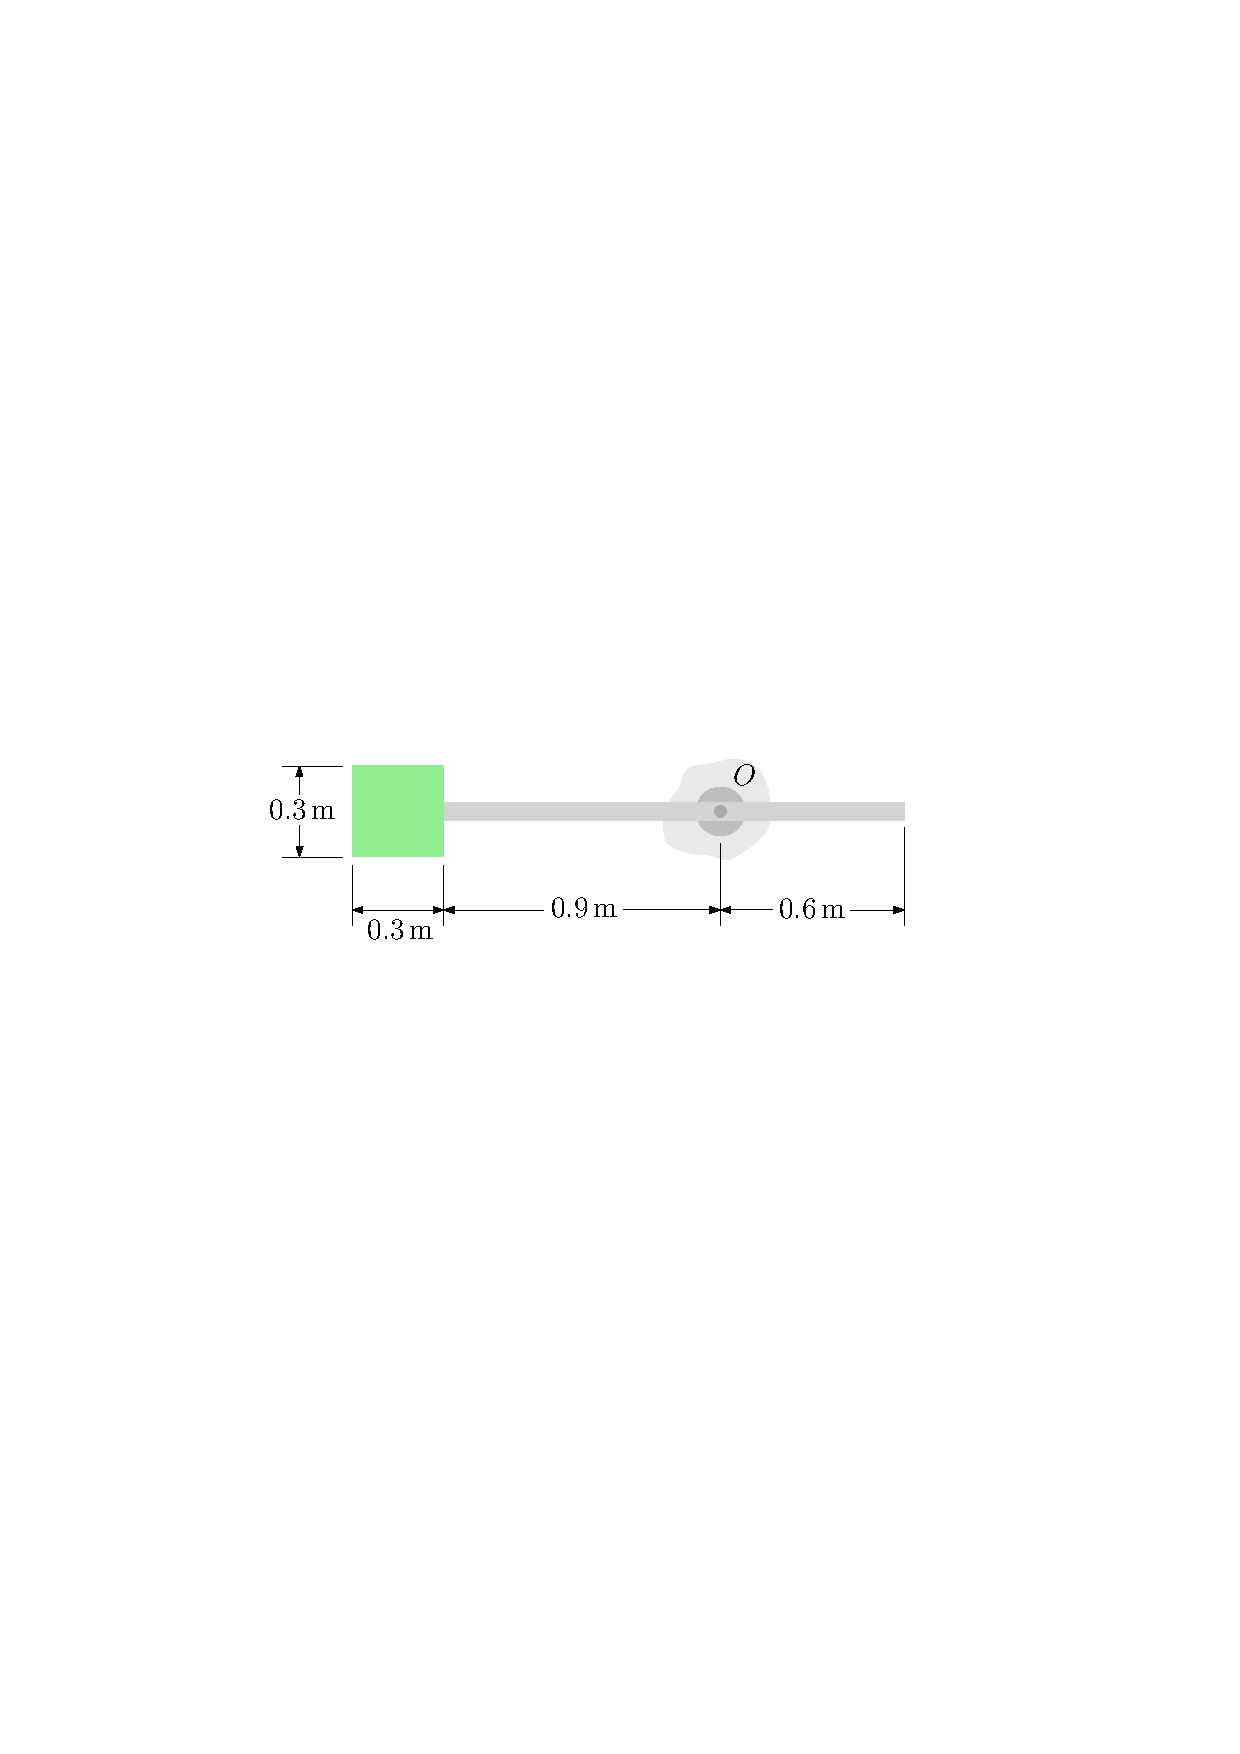
\includegraphics[scale=.9]{../../images/draw_3}
\end{flushright}